%!TEX root = ../Thesis.tex

\chapter{Prototype}
The ground control platform has some physical dimension given due to the size of the UAV used in this project. The dimension of the UAV used will effect the dimension and choice of construction of the ground station. In dimensioning and designing the ground station the primary focus is on making an industrial and robust prototype. 


\section{Landing platform / Helipad}
The landing platform or helipad is a 60cm x 60cm wide plate with a hole in the middle. Dimensioning of the size mainly relies on tolerance on the presision of landing the UAV. The UAV only needs 30cm x 30cm space for the landing gear, but in case a big wind gust comes in just before landing/take-off, the UAV can slide off the platform if the platform is too small. On figure \ref{fig:helipad} the helipad is seen from the top.

\begin{figure}[H]
\centering
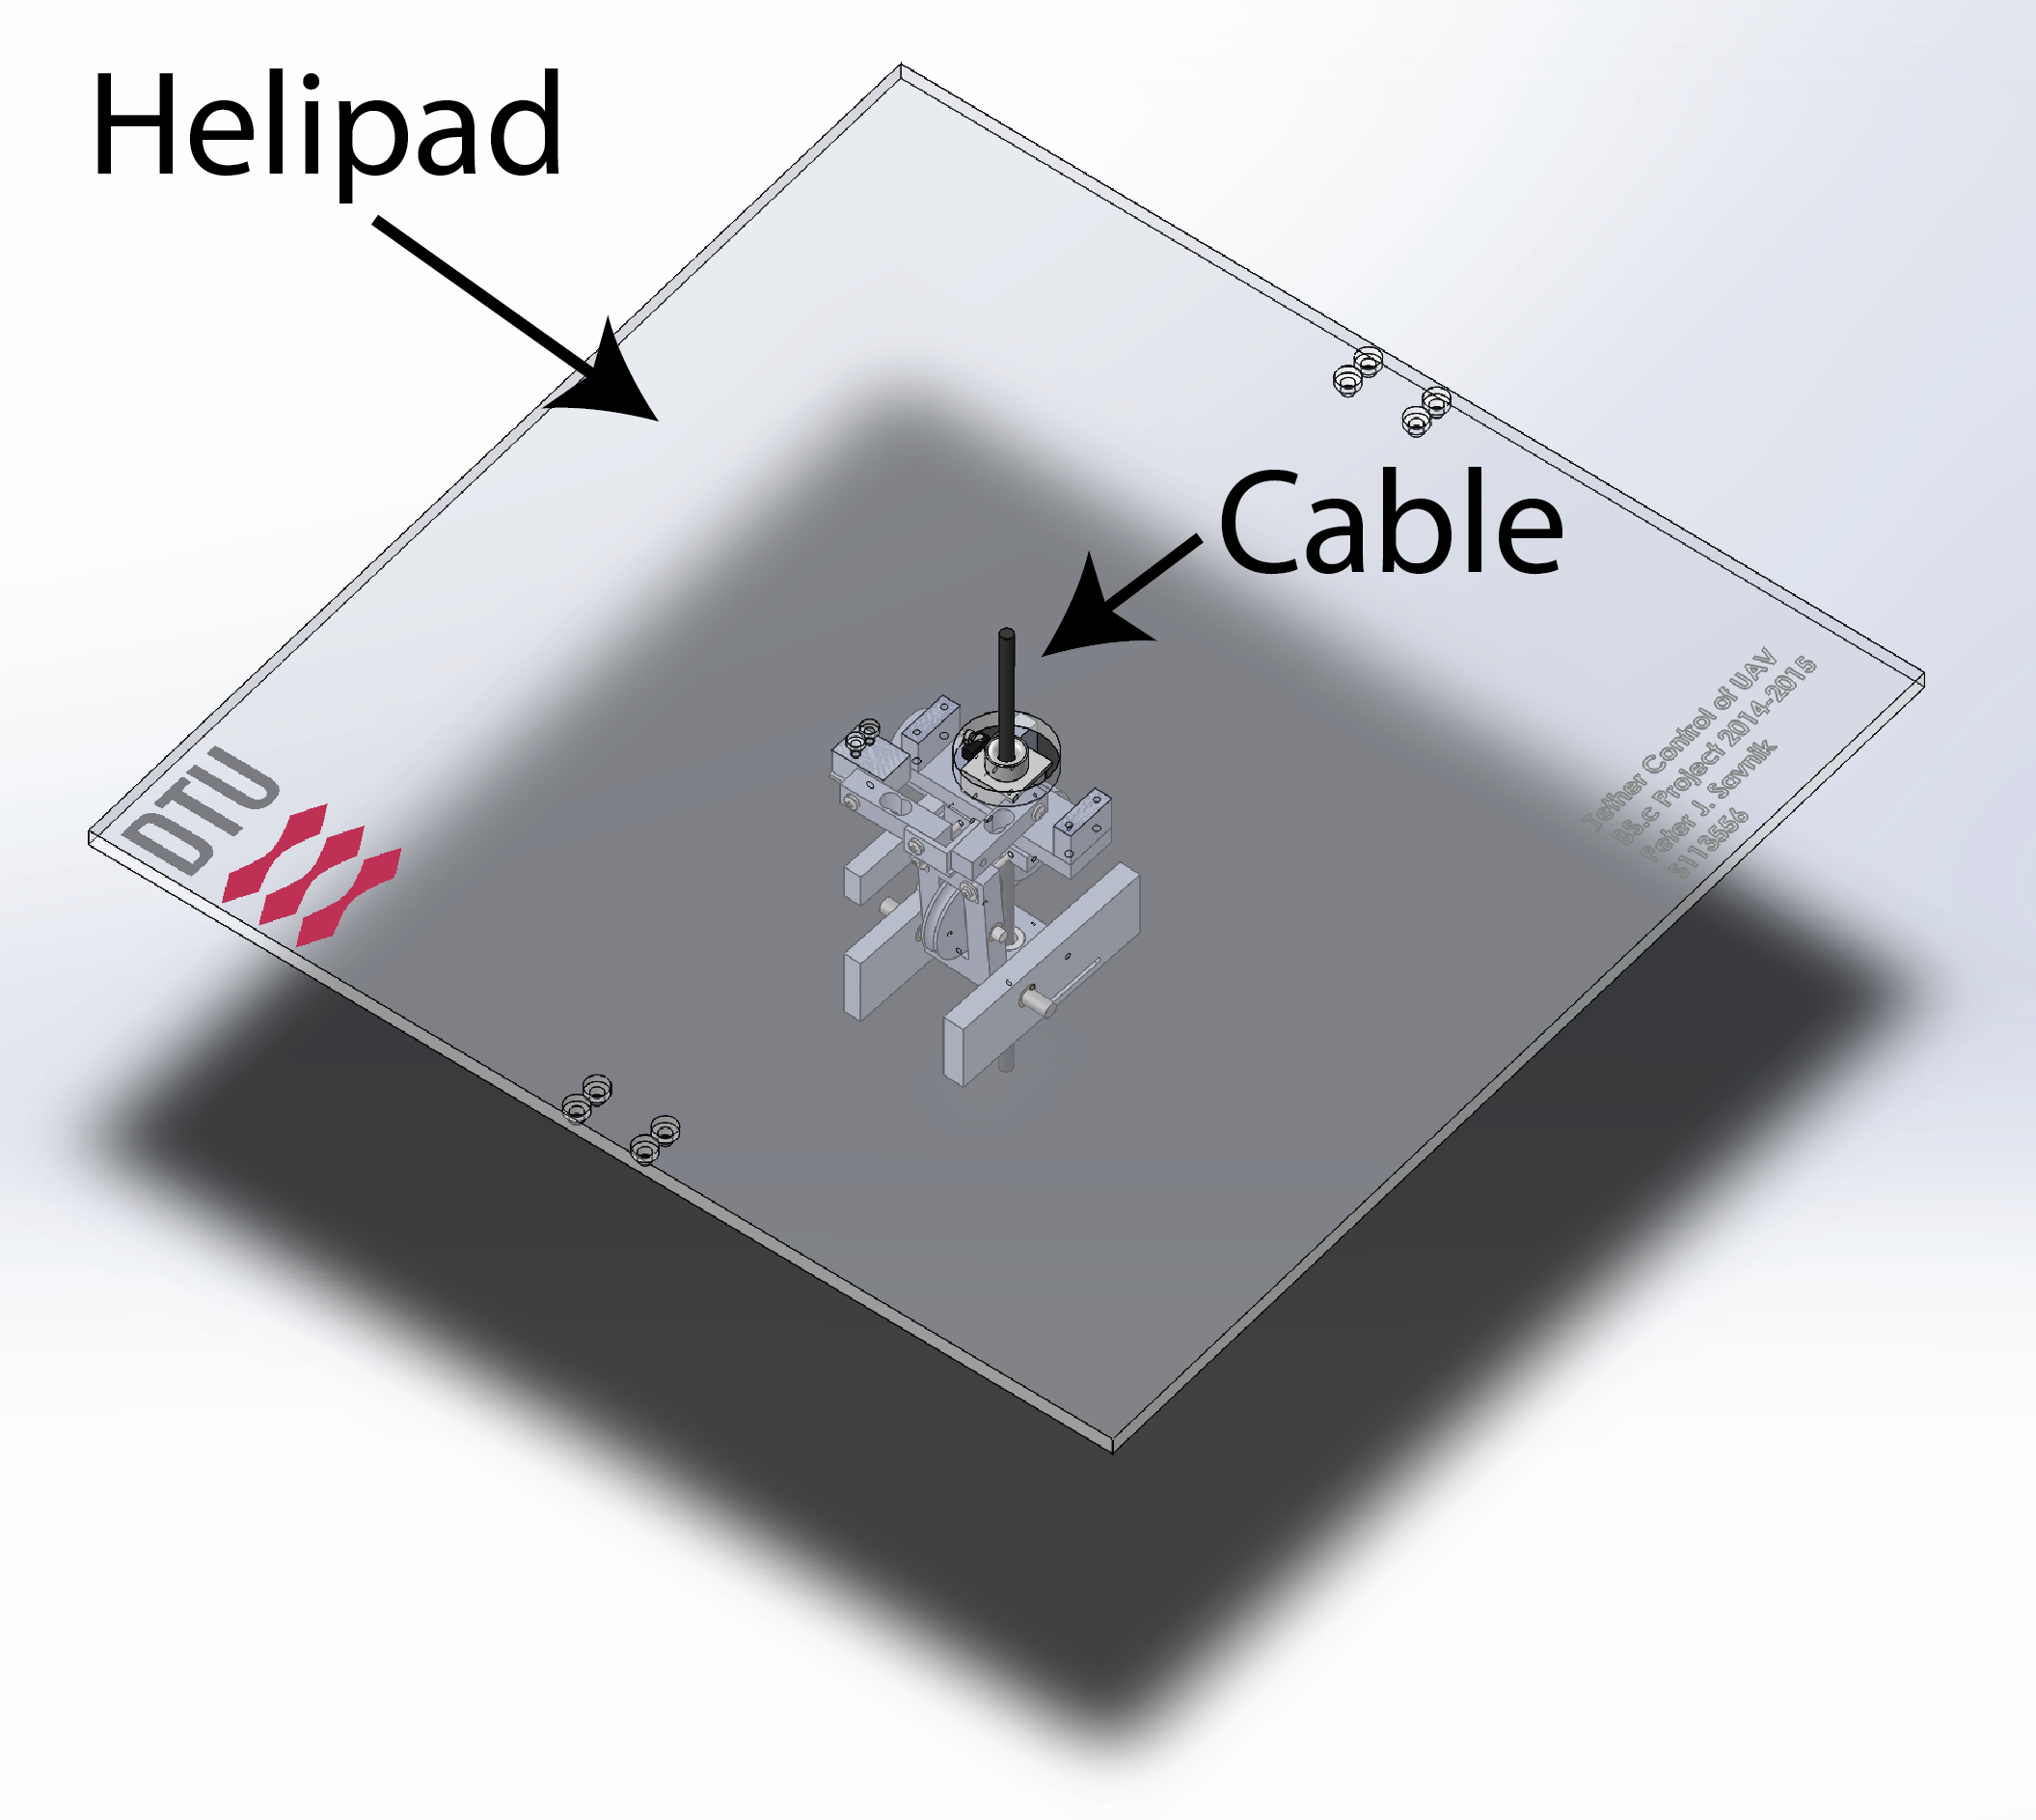
\includegraphics[scale=0.75]{graphics/cad/toplevel.png}
\caption{Illustration of Helipad with a hole in the middle for the cable.}
\label{fig:helipad}
\end{figure}

\section{Messuring the horisontal angle}
In order to precisely determinate where the UAV are positioned relative to the helipad on a horizontal plane a coordinate system on figure \ref{fig:top-coordinates} is introduced. x and y are cartasian coordinates corresponding to the measurements of loadcell 1 and loadcell 2 from figure \ref{fig:loadcells}. $\phi$ is the angle, starting at the positive x direction and increases in positive direction of rotation.

\begin{figure}[H]
\centering
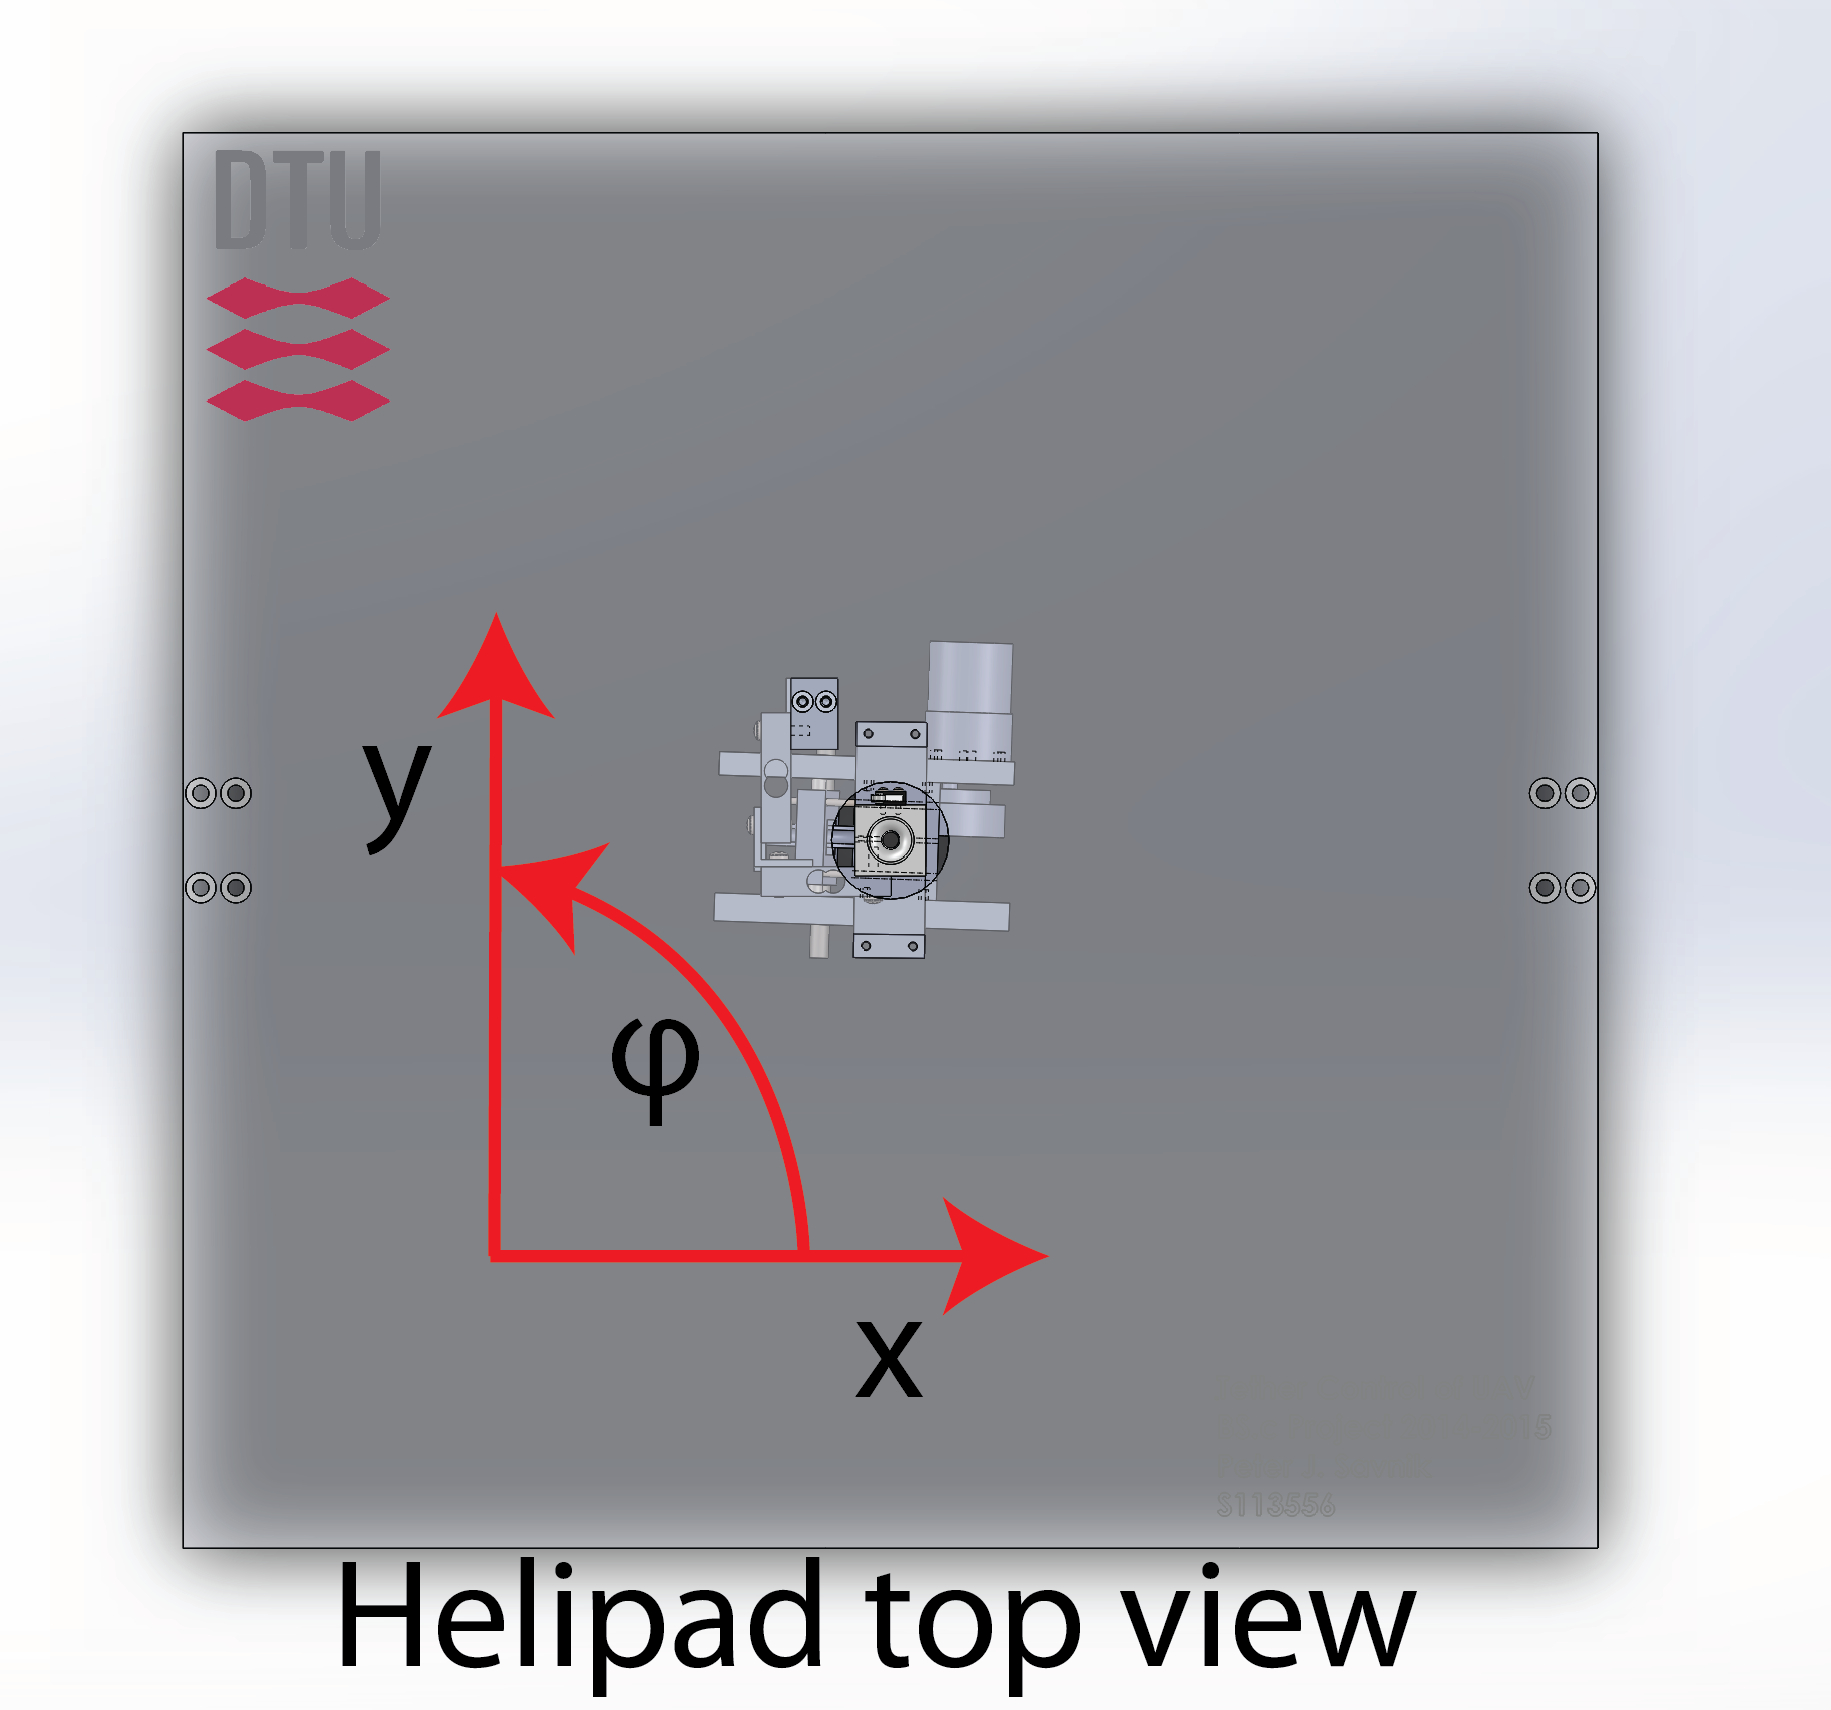
\includegraphics[scale=0.75]{graphics/cad/top-coordinates.png}
\caption{Helipad seen from top view with coordinate system.}
\label{fig:top-coordinates}
\end{figure}

\noindent
To measure the horizontal angle between the ground station and the UAV to loadcells are used, perpendicular to each other. One end attached to the ground station and the other end attached to a cable though hole made in Teflon. Then the UAV is exactly direct over the hole, no force will be measured, but at the UAV moves to one of the sides it will create a cable tension that results in a force in x- and y- direction. Combining the x and y force can be translated to an angle. 

\begin{figure}[H]
\centering
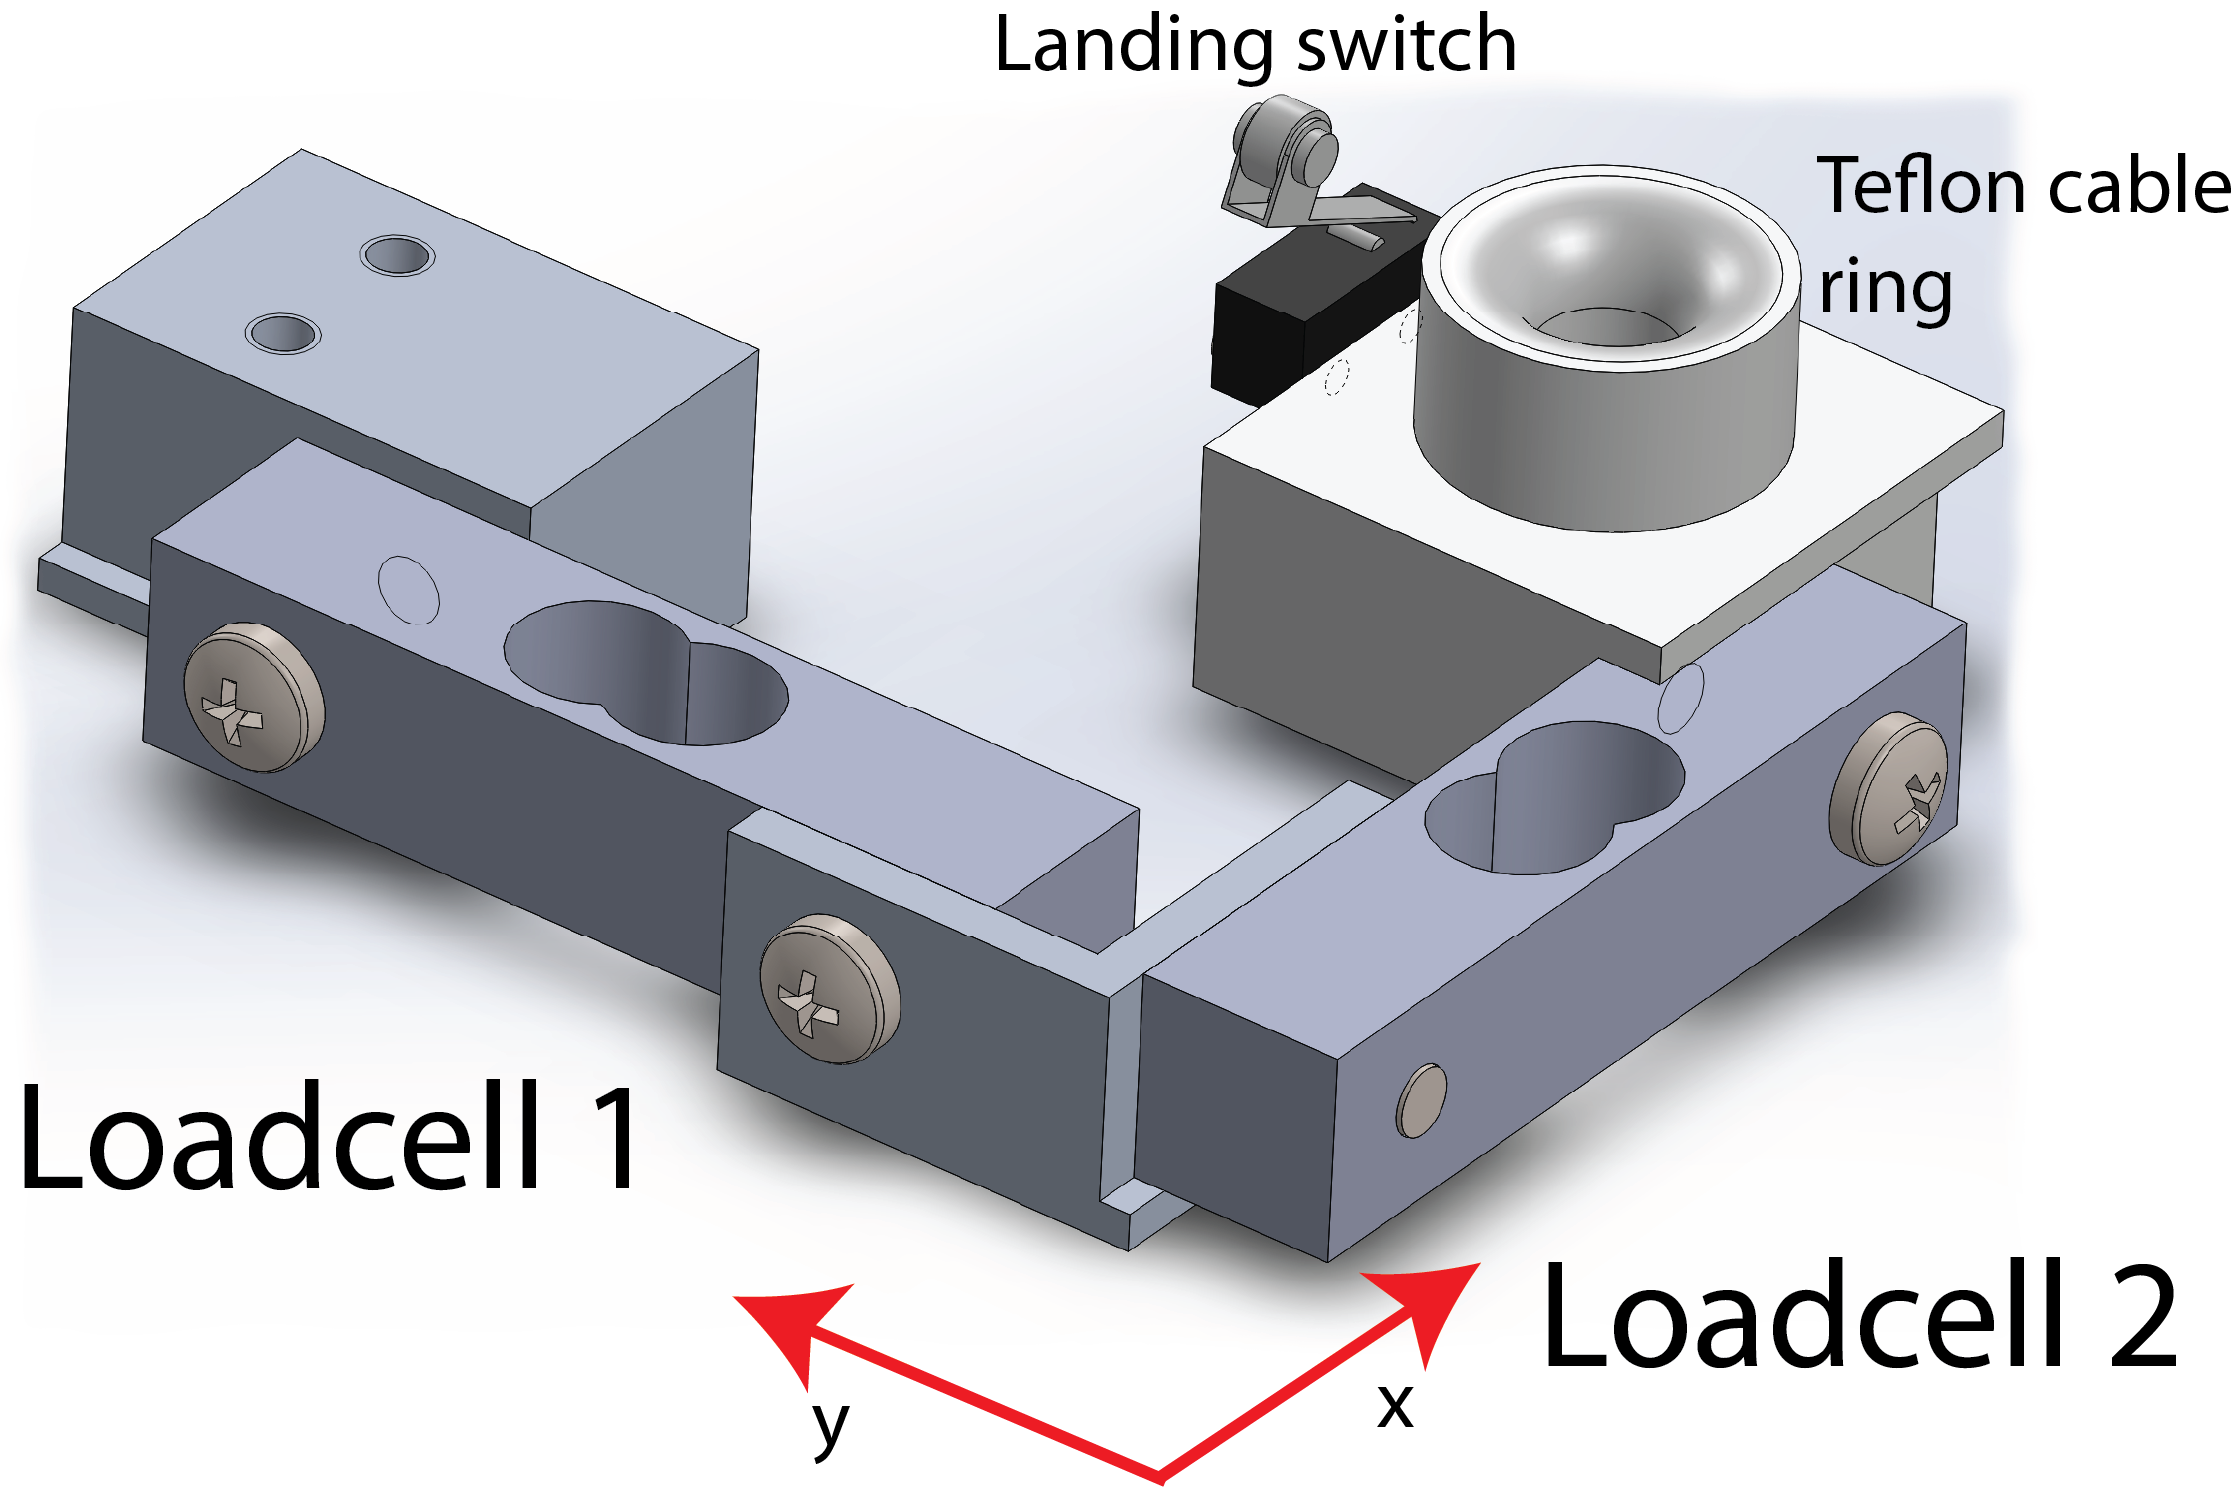
\includegraphics[scale=0.75]{graphics/cad/loadcell.png}
\caption{Configuration of 2 loadcells, for measuring the cable drag in x and y direction. Loadcell 1 measures in x-direction and loadcell 2 in y-direction.}
\label{fig:loadcells}
\end{figure}

\noindent
The UAV can lift about 3kg payload and therefore exert 3kg thrust to the cable and the measuring device must be able to withstand such a force without permanently bending. Two 5kg loadcells from Phidget Inc is assessed to be the best match for the job with regard to what's available in the projects price range.

\subsection{Testing}
First off is calibrating the loadcells. First measurement is without any forces acting in x and y direction in order to determine the offset of each loadcell.
The offset for x is found to $-455.9787$ and the y offset to $-511.2618$.\\
Next 1000g of load is put on the loadcell with a rope through the Teflon ring first purely in positive x direction and next in purely y direction, in order to determine the gain factor $Kx$ and $Ky$. $Kx$ is found to $0.4786$ and $Ky$ to $-0.5134$. Afterwards the calibration is tested by applying a known force in a direction and then checking the result.

\todo{Indsæt figur} 

Second test is done by applying a known force in a combination of x and y direction. For this test $\phi$ is set to 45 degrees and the total force is $1$kg.

\todo{Indsæt figur}


\noindent
Second test was done keeping the $\phi$ angle and the tension constant and varying the $\theta$ angle. Is is expected as $\theta$ approach $90$ degrees the measured force will be approaching $0$. 
\begin{figure}[H]
\centering
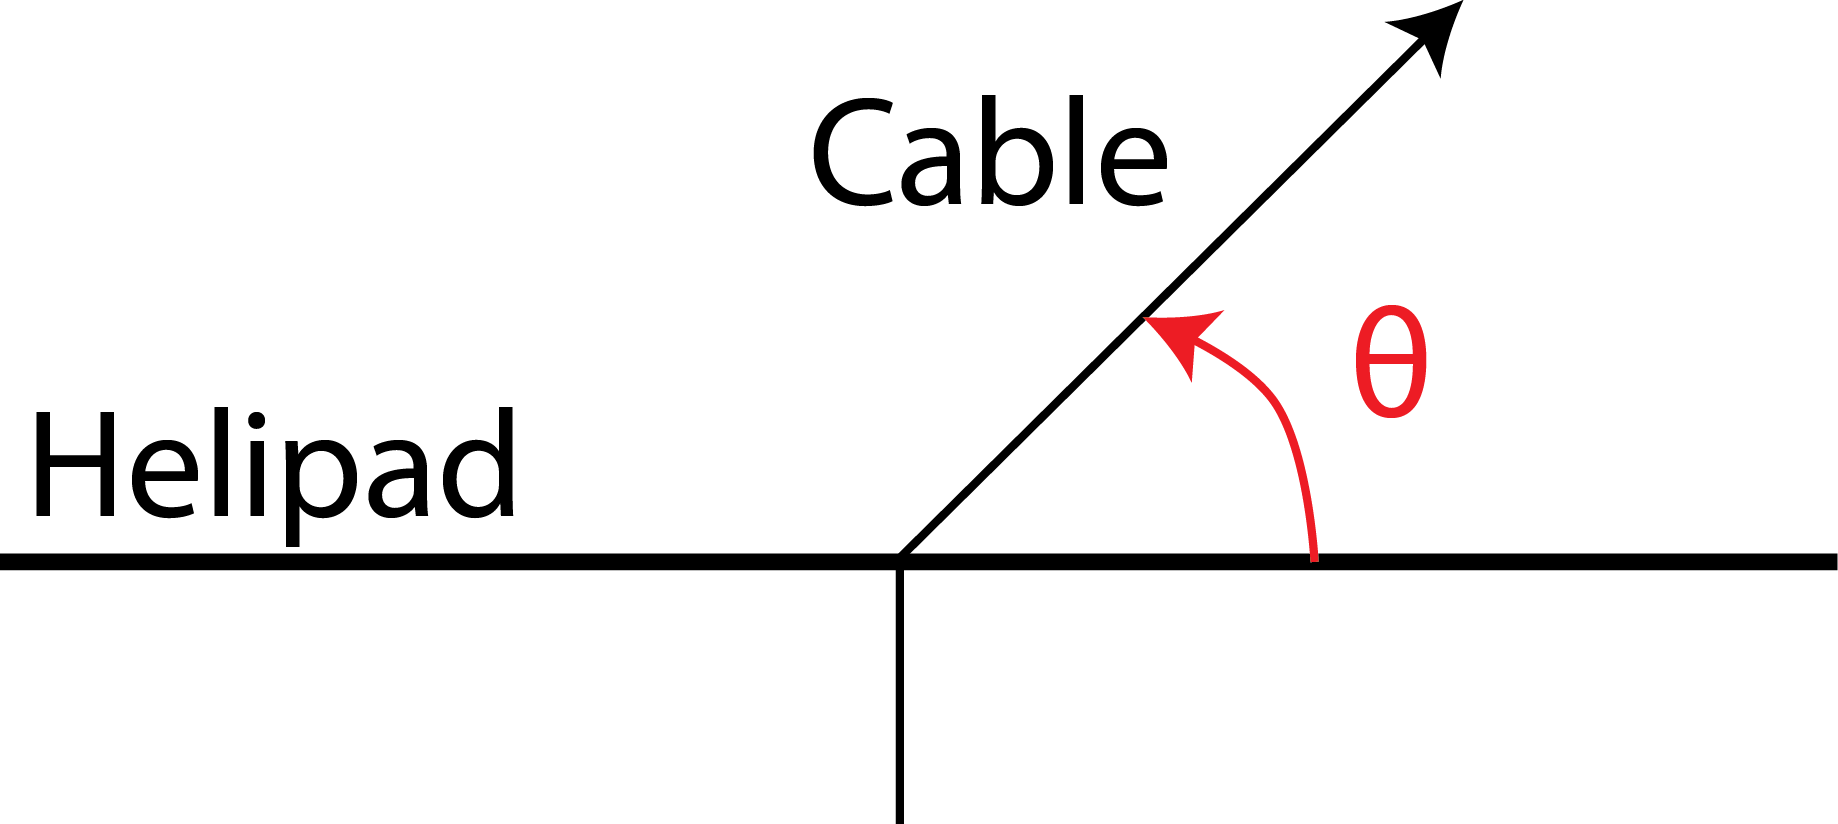
\includegraphics[scale=0.75]{graphics/loadcell_test2.png}
\caption{Testing the horizontal measuring device by keeping $\phi$ constant and varying $\theta$.}
\label{fig:loadcell_test2}
\end{figure}

\noindent
Third test was done in the final assembly and with a real cable. In this test the cable was anchored to the winch below instead of the Teflon ring. This test may vary both $\phi$ and $\theta$.
\todo{Indsæt måle data}
\noindent


\subsection{Summary}
The prototype is able to measure the force in x- and y-direction and $\phi$ can be calculated. \\
\noindent
It turns out that the force applied to both loadcells is much less than expected and is out of range for a 5kg loadcell. The 5kg loadcell has a zero balance at $\pm75g$. If the force is greater the loadcell measurement is out of the zero balance range the device works. Thus, it can reasonably be assumed the devices will work well with a loadcell with a less operating range and higher precision.  
\todo{Kalibrer og find ud af hvor lidt trækket er} 




\section{Winching and storing the cable}
There is several ways to keep the cable when it's not rolled out, 2 commonly used methods are on a cable drum or in a winded pile. The critical parameter here is the flexibility of the cable, diameter of the cable and heat tolerances.  Because the cabled is stored tightly together, heating from the cable resistance has to be given a thought in the cable storing design.

\subsection{Storing cable on a drum}
Storing cable on a drum is a very practical and commonly known method to store cables in a organised way. The benefits of this design is that the drum it self can be used as a winch to winch in the cable. But the minimum diameter of the drum is given by the cable minimum bending radius for flexible installation and that sets a physical minimum for the drums outer diameter. The larger the diameter the greater the force needed for rotating the drum. To assure smooth windings the drum can move from side to side. Physics says the movement from side to side will come natural, if the friction is low enough; in practise this concept works often but is not robust and that is why motorized guidance is needed. In theory the rotation of the drum can be used as a feedback for how much cable is rolled out, but in practice this will be a source to a great error. Further more this design is very dependent on the cable all ways has tension. If there is no or too little tension on the cable it will loosen from the drum. \\
On figure \ref{fig:cable-drum} a cable drum is put under the helipad and the horizontal measurement device. 

\begin{figure}[H]
\centering
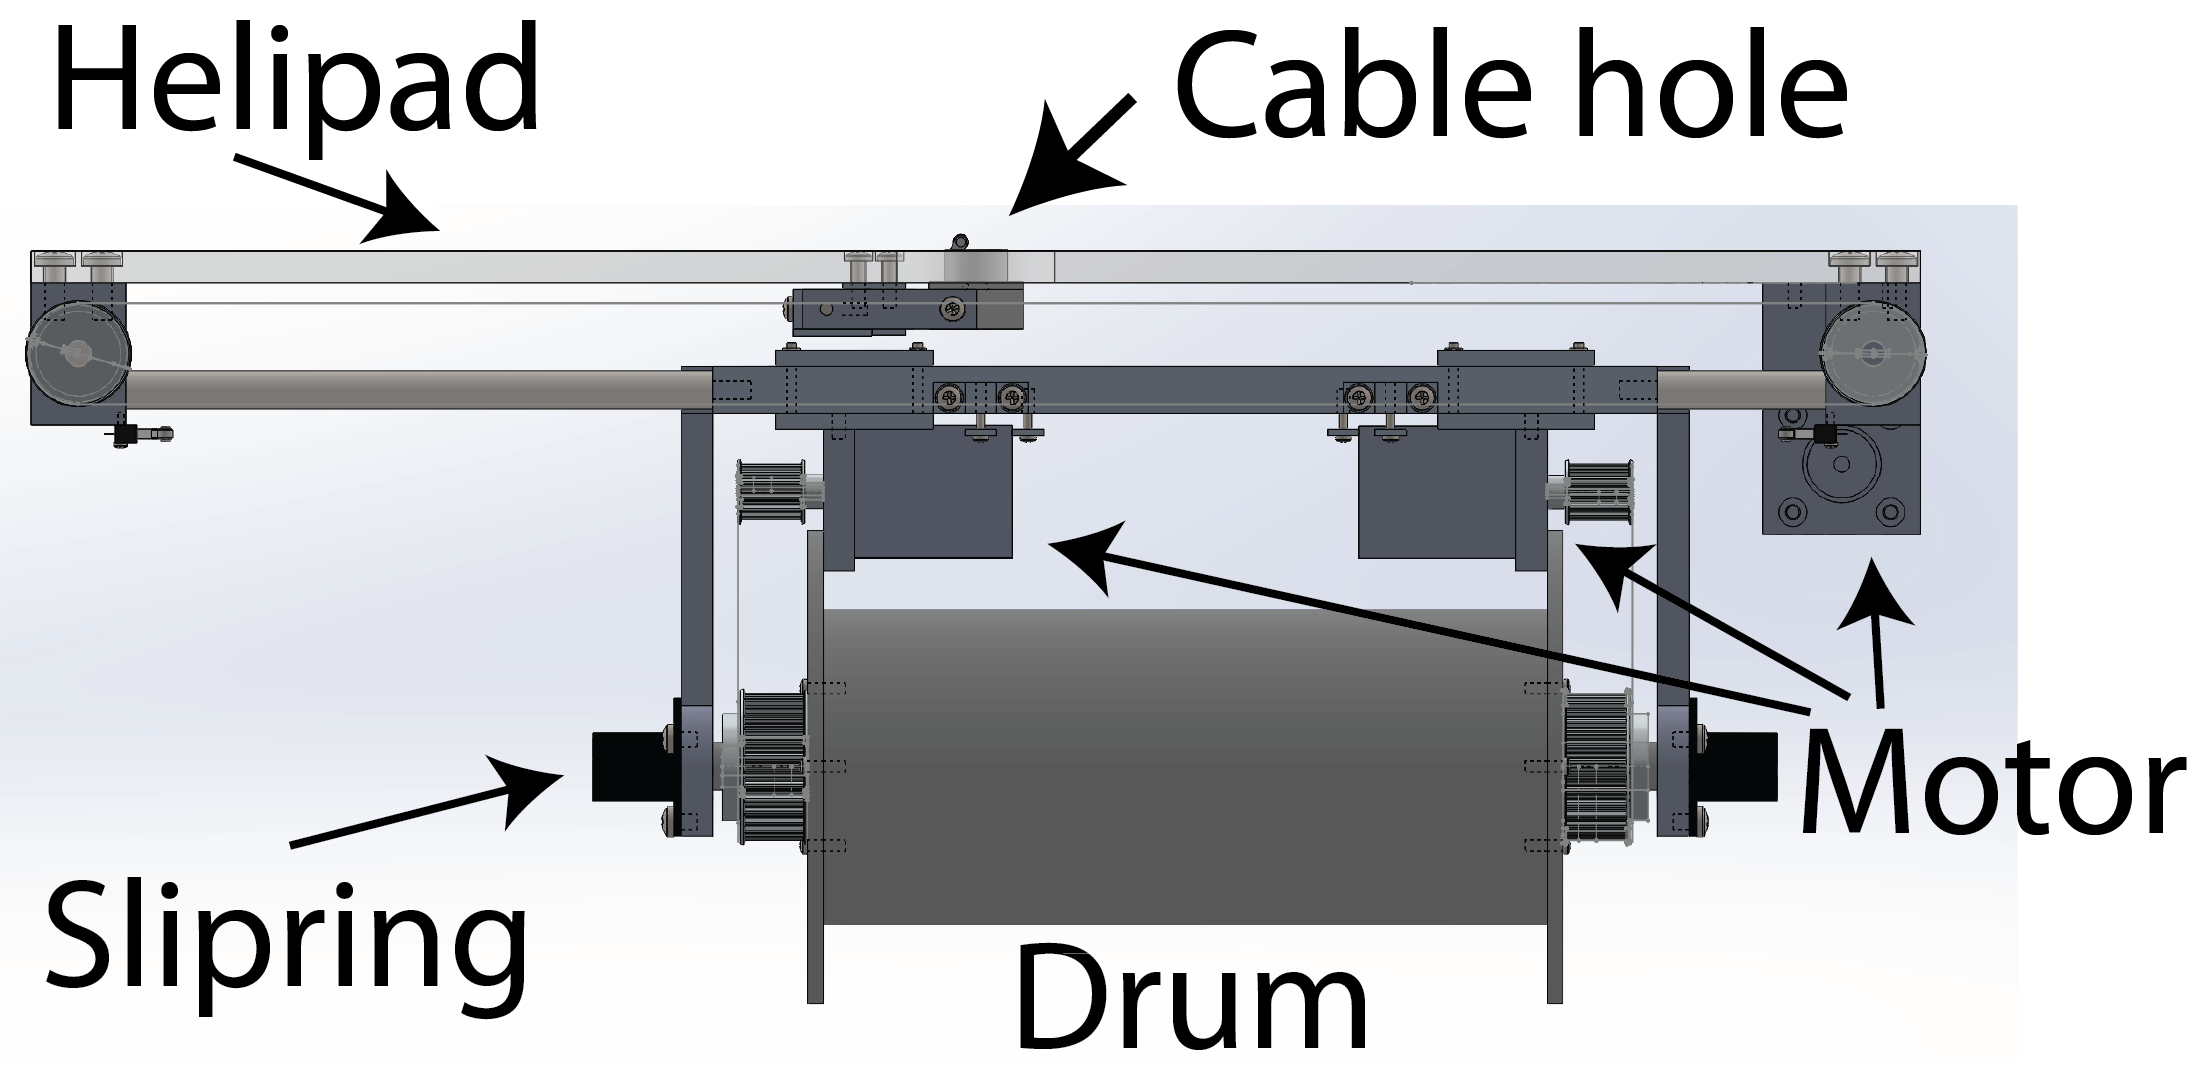
\includegraphics[scale=0.75]{graphics/cad/cable-drum.png}
\caption{Cable drum design. The drum can rotate to winch in/out the cable, and also move from side-to-side to assure smooth windings.}
\label{fig:cable-drum}
\end{figure}

\noindent
With all wire winded in and the UAV on maximum throttle there is assumed to be 500W running through the cable with a electrical loss of around 120 Watt, which is transformed into heat. 120 Watt of heat will give rise to heating up the cable drum. This is a known cause of electrical fire, when a cable drum gets too hot and melts. Therefore a series of pretests where performed to address how big a problem this would bee and too incorporate the result in the design of the system. 

\noindent
The worst-case test with full load over long time was performed at indoor environment with room temperature on 24 degree Celsius. The coil was excited with 75V DC and 30A just over an hour. The inner diameter of the coil is 10cm and is made of 2mm thick PVC pipe.

\begin{figure}[H]
   \centering
   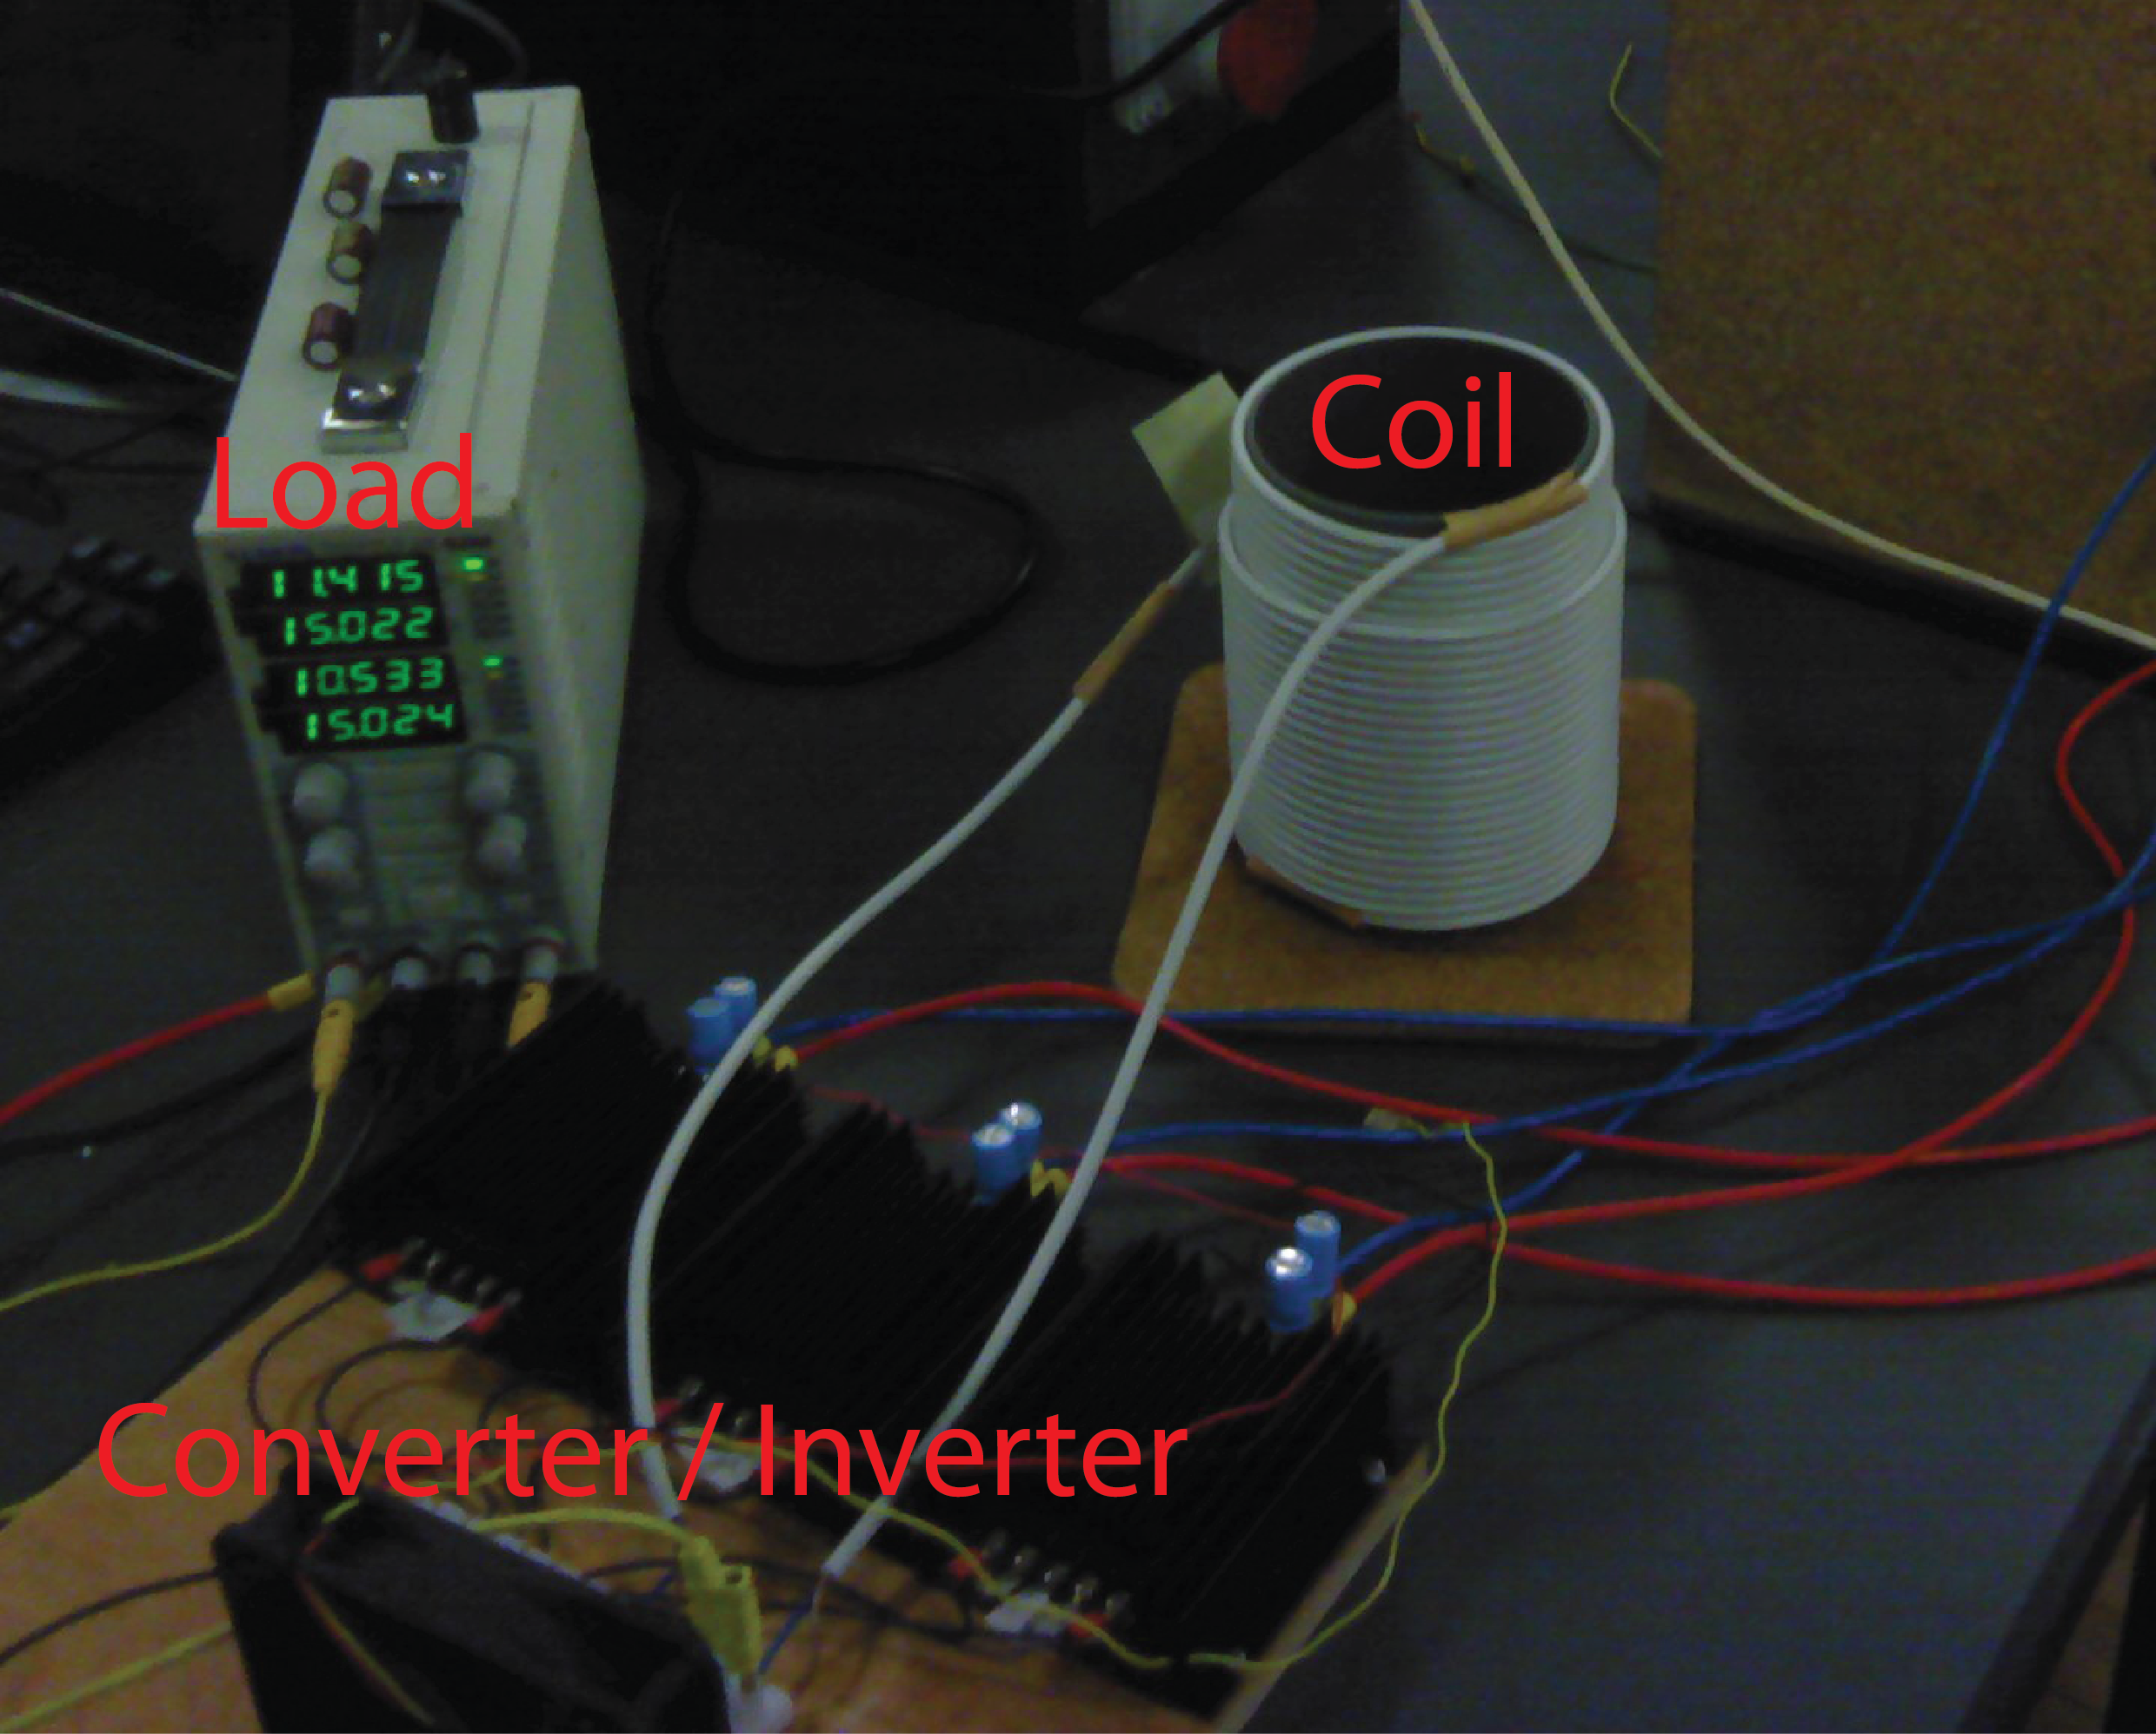
\includegraphics[scale=0.5]{graphics/heat_test/heat_test_setup.png}
   \caption{Heat test setup showing the coil, the test load and power Converters.}
   \end{figure}
      

\begin{figure}[H]
\centering
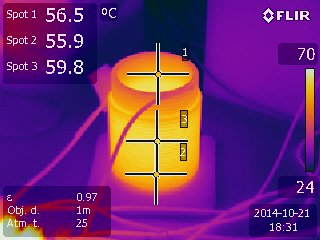
\includegraphics[scale=1]{graphics/heat_test/IR_1491.jpg}
\caption[Caption for LOF]{Heat test of 20m standard household cable\footnotemark winded in 2 layers with 75V DC and 30A. Spot 1 is inside the coil, spot 2 is the lower side of the outer coil and spot 3 i at center of the outer coil. On the lower left corner thermometer calibration constants is displayed.}
\label{fig:heat_test_ir}
\end{figure}
\footnotetext{House hold cable with unknown origin, cross-sectional area 0.75mm2, Max voltage 230 AC, Max current 10A}

\todo{Lav matlab plot af data}

\subsection{The Simple Winch}
Sometimes simple is better. The simple design has a motorized toothed wheel and an encoder wheel pushing the cable against the motorized wheel. The encoder wheel turns only when the cable is moving, and the slip is minimal making it a very robust feedback for the motor controller. The encoder wheel is pushing the cable toward the motor wheel with a spring, that assures small imperfections in the cable does not make it slip. two simple screws adjust the spring tension. For storing the cable a box underneath collects the cable.

\begin{figure}[H]
\centering
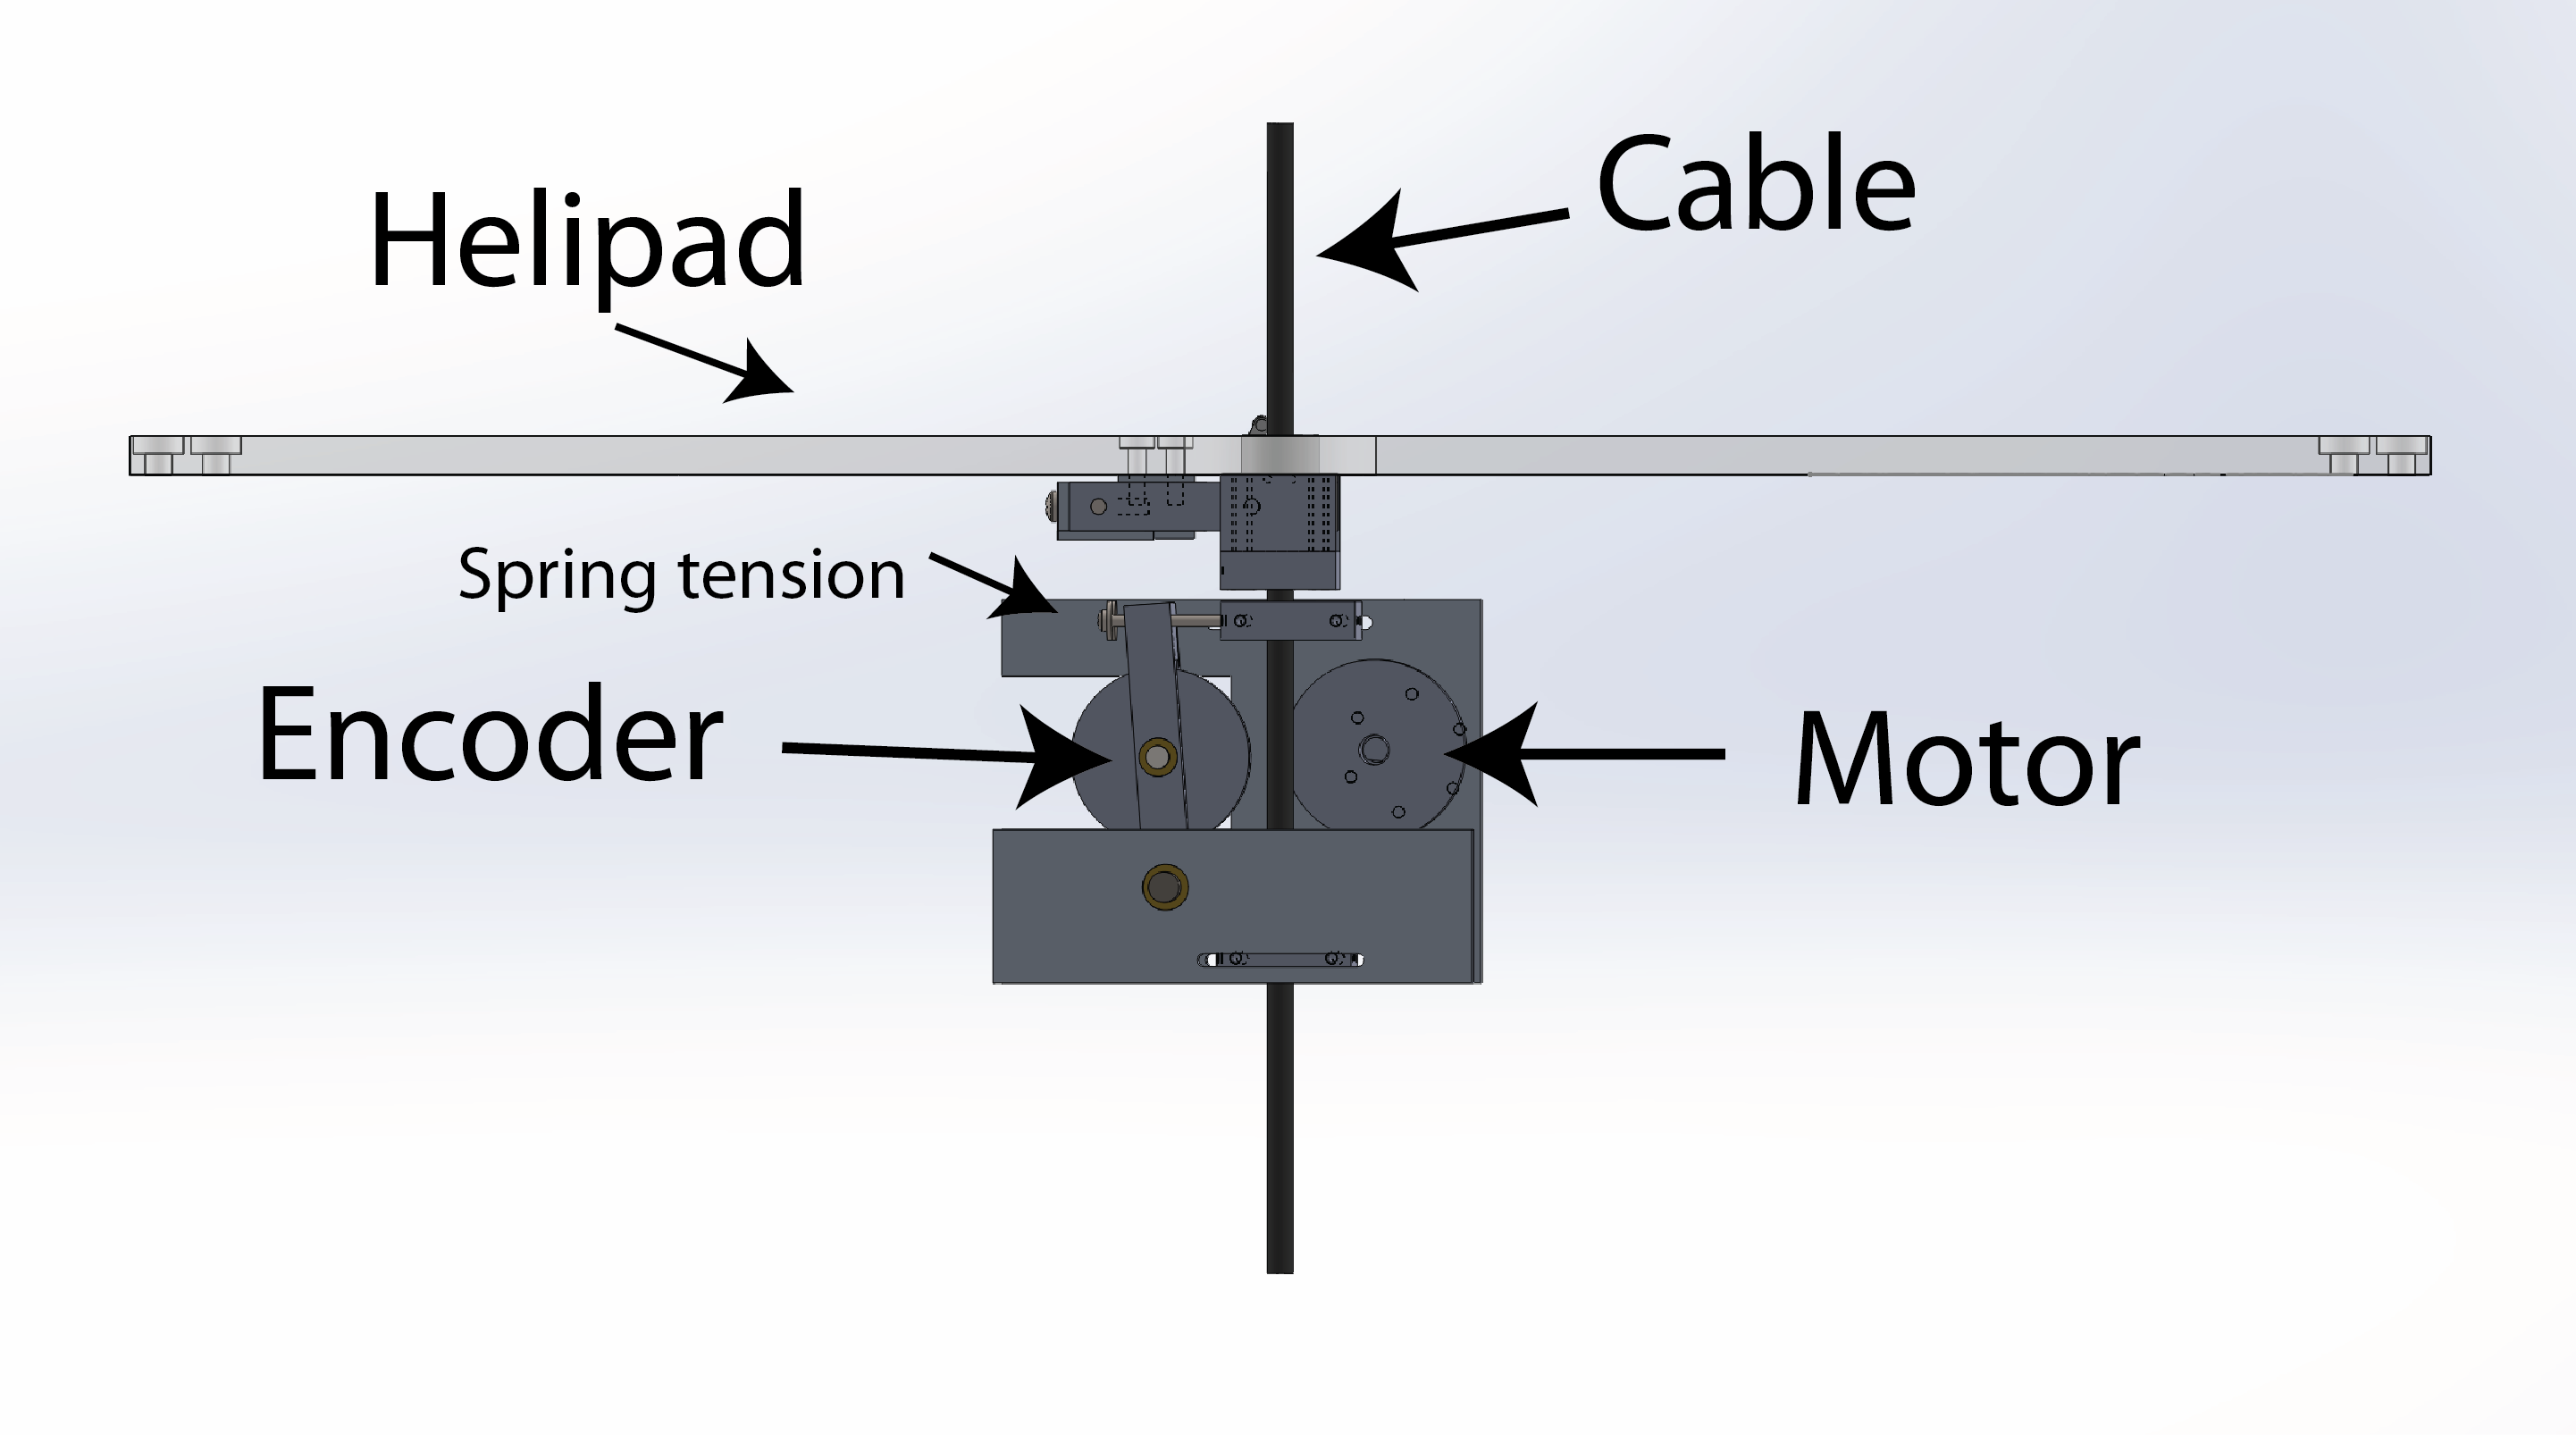
\includegraphics[scale=0.75]{graphics/cad/winch.png}
\caption{The Simple Winch only has one motor and an encoder wheel pushing the cable towards the motor wheel. Two springs adjust the tension.}
\label{fig:winch}
\end{figure}

\subsection{Comparison}
Both concepts are mature enough to be prototyped and tested, but due to the time frame of this work there is only time for manufacturing and testing one design. Based on the lower mechanical complexity of the simple winch, the simple winch is the chosen design.    


\section{Cable Connection to the UAV}
Connecting the cable to the UAV has several issues to address. First a 3-axis measurement device is needed to measure how much the cable tension is and in which direction. Second a connector 





\section{Electrical Design}
From an electrical view there are 2 separate systems, Flight Control System on the UAV and Ground Control Station. The system reading the sensor data on the Ground Control Station has to feed the UAV with the measured data hence the UAV's possession controller is running on the UAV. 

\todo{Wire diagram der viser system overview}

\subsection{Ground Station}
The ground station sends data to the UAV system and decides weather to roll cable in or out based on the wanted position. The control of feeding the cable is done by comparing the load on the UAV system to what is expected by the weight of the rolled out amount of cable. If the load is higher then expected more cable are rolled out and vice versa.  


\subsection{UAV System}
The system on the UAV measures a 3-axis loadcell connected to a Phigets Bridge. The Phidget Bridge are interfaced via a Beaglebone Black.  




\section{Software design}


\subsection{Flight Control System}


\subsection{Ground Control Station}
